\chapter{Graphical design}
The graphical user interface is what most users of a system interacts with. Therefore, it is important that the user interface is well designed, responsive and intuitive. With a good design, the users can work more effectively on the system, and not be confused by the layout. In order to make a great design, the designer have to really think about all the aspects with the design. Who is the user of the system? What should the user interface provide to the user? What should the user interface communicate? These are some of the questions that needs to be answered.
\\\\
The group, with some input from the customer, tried to make the user interface as intuitive, and clean and simple as possible.

\section{Planning of design}
The customer gave the group a design manual, which included what colors to use, guidelines for using their logo, and other general design related matters. The customer didn't have any design proposals, and gave the group a relatively open task. They did, however, have a few inputs on the target audience, which was going to be children between six and ten years. From this information, some assumptions could be made:\\
\\

\begin{itemize}
  \item The application interface has to be simple and intuitive
  \item The colors, and graphics should be ``childish", and child-engaging
  \item All information presented in the application should be written in a language targeting children.
\end{itemize}

The group spent the first weeks designing, and improving their starting ideas. After some discussion within the group, some clear points of design had been made, based on user interface design basics. \cite{uidesignbasics}

\begin{itemize}
  \item The interface should be consistent, and use common user interface elements, such as a standard menu button, and standard page-navigation inside the application.  
  
  \item The application should have a design with a purpose, and elements should be logically placed throughout the application
  
  \item Fonts, and font sizes should be used as a tool, to create a sense of hierarchy and structure.
  
  \item The users should not wander in the dark. It is important to provide the user with enough information to understand how they are supposed to use the application. The text and buttons should be explained precise enough for the user to know what the next step is.
  
  \item The system should also communicate what is happening. If a button is pressed, or a setting is switched, the system should give some kind of feedback, so the user knows that the program has responded.
\end{itemize}

\section{Designing the application}
The first few weeks was used to make a good design the group, and the customer was satisfied with. The elements that were designed 

\subsection{Sketches}
The group discussed the outline of the different parts of the application, and made some rough sketches to have something to start from. When these sketches were done, it was shown to the customer, and they gave their approval of the ideas, and outline of the general design. The first designdrafts can be seen in figure \ref{fig:welcomeScreen} - \ref{fig:memoryMinigame}

\begin{figure}[H]
  \begin{minipage}[t]{0.35\textwidth}
    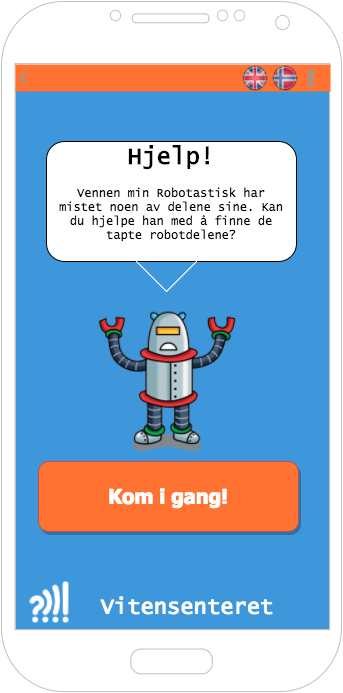
\includegraphics[width=\textwidth]{images/sketches/Welcome.png}
    \caption{Welcome Screen}
    \label{fig:welcomeScreen}
  \end{minipage}
  \hfill
  \begin{minipage}[t]{0.35\textwidth}
    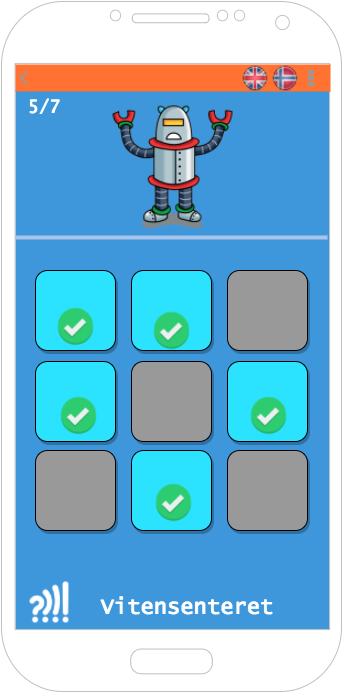
\includegraphics[width=\textwidth]{images/sketches/MainScreen.png}
    \caption{Overview screen}
  \end{minipage}
\end{figure}

\begin{figure}[H]
  
  \begin{minipage}[b]{0.35\textwidth}
    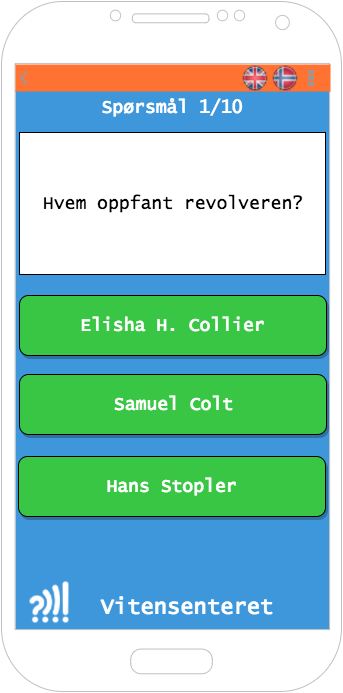
\includegraphics[width=\textwidth]{images/sketches/quiz.png}
    \caption{Quiz minigame}
  \end{minipage}
  \hfill
  \begin{minipage}[b]{0.35\textwidth}
    \includegraphics[width=\textwidth]{images/sketches/ShortestPath.png}
    \caption{Shortest path minigame}
  \end{minipage}
  \begin{minipage}[b]{0.35\textwidth}
    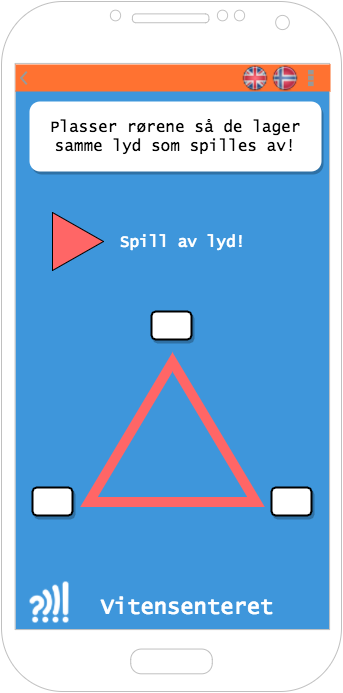
\includegraphics[width=\textwidth]{images/sketches/SoundGaem.png}
    \caption{Sound minigame}
  \end{minipage}
  \hfill
  \begin{minipage}[b]{0.35\textwidth}
    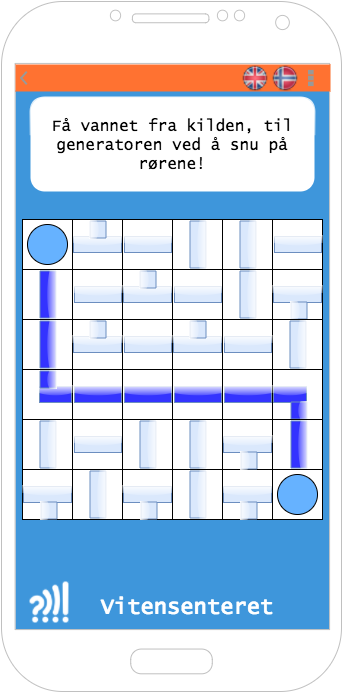
\includegraphics[width=\textwidth]{images/sketches/WaterFlow.png}
    \caption{Waterflow minigame}
  \end{minipage}
\end{figure}

\begin{figure}[H]
  \begin{minipage}[b]{0.35\textwidth}
    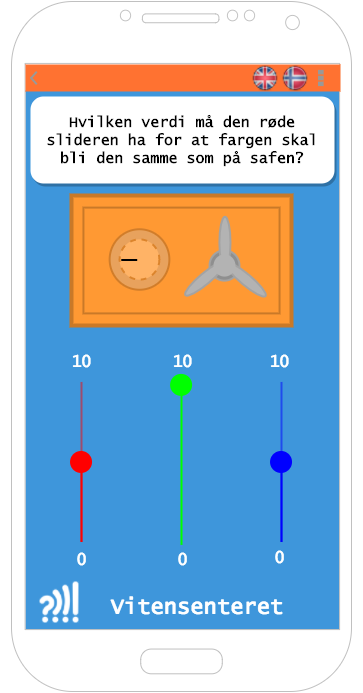
\includegraphics[width=\textwidth]{images/sketches/ColorSlider.png}
    \caption{Color slider minigame}
  \end{minipage}
  \hfill
  \begin{minipage}[b]{0.33\textwidth}
    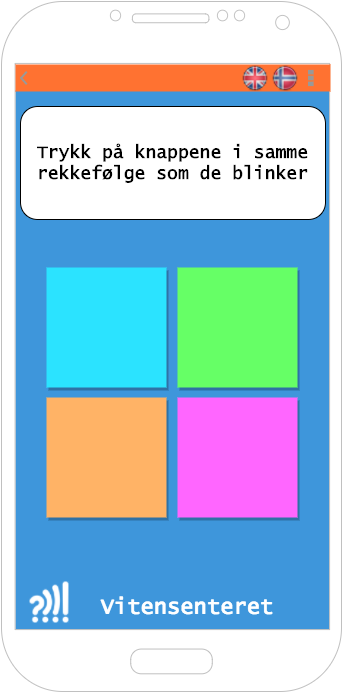
\includegraphics[width=\textwidth]{images/sketches/MemoryGame.png}
    \caption{Memory minigame}
    \label{fig:memoryMinigame}
  \end{minipage}
\end{figure}

\section{Changes in design}
Some changes were made in the final version to make the process more effective for the group. By using the built-in user interface elements from the framework, the group could do the development of the graphical design faster than by designing all user interface elements from scratch(e.g. popup menus, information cards). Even though some changes had to be made, but the idea, and principles are the same as in the first drafts.
\\\\
Since the implementation of flat design is getting more popular, the group decided to go for this design approach. By doing this, the application is following the evolution of popular design trends, and makes the application up to date on the design-front. It makes the application seem more simplistic, but preserves the functionality.



\begin{figure}[H]
  \begin{minipage}[b]{0.35\textwidth}
    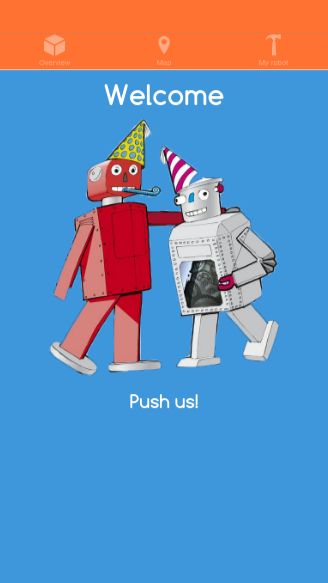
\includegraphics[width=\textwidth]{images/app/welcomeScreen.png}
    \caption{Welcome Screen}
  \end{minipage}
  \hfill
  \begin{minipage}[b]{0.35\textwidth}
    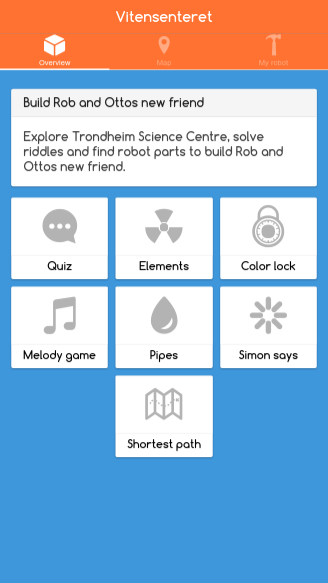
\includegraphics[width=\textwidth]{images/app/overview.png}
    \caption{Robot part main screen}
  \end{minipage}
  \begin{minipage}[b]{0.35\textwidth}
    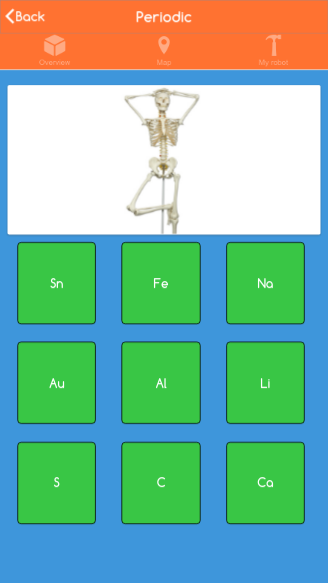
\includegraphics[width=\textwidth]{images/app/Periodic.png}
    \caption{Table of elements mini-game}
  \end{minipage}
  \hfill
  \begin{minipage}[b]{0.35\textwidth}
    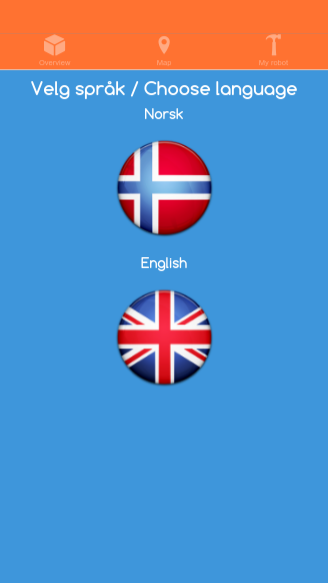
\includegraphics[width=\textwidth]{images/app/chooseLanguage.png}
    \caption{Choose language, welcoming screen}
  \end{minipage}
\end{figure}

\section{Implementation of design}
Design is always a challenge when creating mobile applications, or other programs that needs a user interface. The design has to engage the user, it has to be intuitive, and easy to use. The group found some elements of importance, in order to create a clear, and tidy design.
\\\\
The group followed sketches from the starting phase in the final design. As mentioned in the previous section, some changes were made in the final implementation. This section covers the most important design aspects of the overall design implementation.

\subsection{Fonts}
The application uses one type of font, which is named ``Comfortaa". It is downloaded from Google's font-base, which is free to use. The font is a ``childish" font, which aims to engage the user base of the application.
\\\\
The group strived to use font sizes in a way that made all messages given to the user seem clear. The same font size is used for headlines of a message, to give the user the subject for the message. All other information is written in normal font size. This makes a clear hierarchy, which makes it easy to read the information provided. Some information is written in ``bold" text, to emphasize its importance.

\subsection{Colors} The colors used throughout the application is chosen from Vitensenterets color-palette. The main colors used are orange, green, and red. The usage of colors are carefully thought through. Buttons that indicate an ``OK" or ``Move on", are green. Messages indicating the opposite are red. The reason for this choice, is that most signs, or signals that is green, indicates a ``go", while red indicates ``stop". The color complements the text on the button, giving the user a visual representation of the action to be made. 
\\\\
In order to give the user a visual feedback when pressing on a button, the color of the button becomes darker when pressed.

\subsection{Complexity} If an application is too intricate, the user might not be comfortable using it. The goal of the design is to provide the user with the exact amount of information they need, in order to use the application as it is meant to. The design is as simple as it can be, without loosing functionality or playfulness.

\subsection{Graphics}Since the group had a lack of graphical design skills, most of the graphics in the application are designed by Vitensenterets own designer. This gives the customer full control over what graphics that are viewed in the application. There are three elements downloaded from the internet, under the apache licence\cite{apache_licence}, the flags in the language selection, the pipes used in the waterflow game, and the images in the Periodic minigame.

\subsection{Continuity} One of the most important design matters of a user interface, is continuity. By making a template for buttons, information boxes, and other commonly used elements in an application makes it easier to understand the flow of the program. If the user recognizes a pattern, it is easier to get used to the application, and thus, it does not confuse the user. The group made templates for all information cards, buttons, and pop-ups, in order to maintain a continuous design throughout the application.


\subsection{Logic}
When selecting colors for the application the group chose the colors from Vitensenteret's color pallette which were strong and complimentary to each other. An example of this are the primary light-blue and orange which are used as background and foreground colors.\\\\
The buttons were made big and simple, so that the intended user group, children aged 6-10 years, would be able to press them easily. Some changes were made to the original design, removing or thinning black borders around elements. This was done to give the application a more ``professional" and simplistic look, and not as ``toy-like" as the original designs.
